\documentclass[11pt]{standalone}
\usepackage{tikz}
\usepackage{pgfplots}
\usepackage{tikz-3dplot}
\pgfplotsset{compat = 1.9}
\usepackage{amsthm}
\usepackage{amsmath}
\usepackage[english]{babel} 
\usepackage[T1]{fontenc}
\usepackage[utf8x]{inputenc}


\begin{document}

	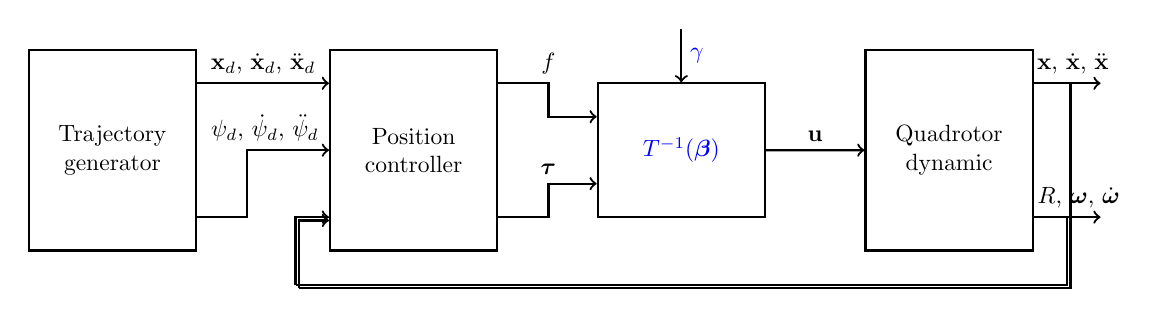
\begin{tikzpicture}[thick,scale=0.85, every node/.style={scale=0.85}]
		\coordinate (origin)  at (0,    0);
		\coordinate (traj)    at (0.5,    1);
		\coordinate (control) at (5,    1);
		\coordinate (mixing)  at (9,    1.5);
		\coordinate (dynamic) at (13,   1);
		\coordinate (output1) at (16.5, 2.5);
		\coordinate (outfit1) at (16,   2.5);
		\coordinate (outfit2) at (4.5,    0.5);
		\coordinate (outfit3) at (4.55,    0.45);

		\node[draw, minimum width=2.5cm, minimum height=3cm, anchor=south west, align=center] (TRA) at (traj) {Trajectory\\generator};
		\node[draw, minimum width=2.5cm, minimum height=3cm, anchor=south west, align=center] (CON) at (control) {Position\\controller};
		\node[draw, minimum width=2.5cm, minimum height=2cm, anchor=south west, align=center] (MIX) at (mixing) {$\textcolor{blue}{T^{-1}(\boldsymbol{\beta})}$};
		\node[draw, minimum width=2.5cm, minimum height=3cm, anchor=south west, align=center] (DYN) at (dynamic) {Quadrotor\\dynamic};

		\draw[->] ($(TRA.0)+(0, 1)$) -- node[above]{$\mathbf{x}_d$, $\dot{\mathbf{x}}_d$, $\ddot{\mathbf{x}}_d$} ($(CON.180)+(0, 1)$);
		\draw[->] ($(TRA.0)-(0, 1)$) - ++(0.75, 0) -- ++(0.75, 0) |- node[above]{\hspace{15pt}$\psi_d$, $\dot{\psi}_d$, $\ddot{\psi}_d$} ($(CON.180)$);
		\draw[->] ($(CON.0)+(0, 1)$) - ++(0.75, 0)node[above]{$f$} -- ++(0.75, 0) |- ($(MIX.180)+(0, 0.5)$);
		\draw[->] ($(CON.0)-(0, 1)$) - ++(0.75, 0) -- ++(0.75, 0) |- node[above]{$\boldsymbol{\tau}$} ($(MIX.180)-(0, 0.5)$);
		\draw[->] ($(MIX.0)$) -- node[above]{$\mathbf{u}$} ($(DYN.180)$);
		\draw[->] ($(DYN.0)+(0, 1)$) -- node[above]{\hspace{5pt}$\mathbf{x}$, $\dot{\mathbf{x}}$, $\ddot{\mathbf{x}}$} ($(DYN.0)+(1, 1)$);
		\draw[->] ($(DYN.0)-(0, 1)$) -- node[above]{\hspace{10pt}$R$, $\boldsymbol{\omega}$, $\dot{\boldsymbol{\omega}}$} ($(DYN.0)+(1, -1)$);
		\draw[-] ($(DYN.0)+(0.5, -1)$) |- (outfit2);
		\draw[-] ($(DYN.0)+(0.55, 1)$) |- (outfit3);
		\draw[->] (outfit2) |- ($(CON.180)-(0, 1)$);
		\draw[->] (outfit3) |- ($(CON.180)-(0, 1.05)$);
		\draw[->] ($(MIX.90)+(0, 0.8)$) -- node[right]{$\textcolor{blue}{\gamma}$} ($(MIX.90)$);
		%\draw[-] ($(MIX.90)+(0, 0.8)$) -- ($(CON.90)+(0, 0.3)$);
		%\draw[->] ($(CON.90)+(0, 0.3)$) -- ($(CON.90)$);
 
	\end{tikzpicture}

\end{document}